\documentclass[a4paper,parskip,11pt, DIV12]{scrreprt}
\usepackage[english]{babel} % Für Deutsch [english] zu [ngerman] ändern. 
\usepackage[utf8]{inputenc}
\usepackage[T1]{fontenc}
\usepackage{lmodern}
\usepackage{blindtext}
\usepackage{graphicx}
\usepackage{caption}
\usepackage{subcaption}
%\renewcommand{\familydefault}{\sfdefault}
%\usepackage{helvet}
\usepackage{fancyhdr}
\usepackage{amsmath}
\usepackage{mdwlist} %Benötigt für Abstände in Aufzählungen zu löschen
\usepackage{framed} %Rahmen um Objekte
\usepackage{floatflt} %Text neben Bildern
\usepackage{colortbl} % Tabellen einfärben
\usepackage{here}
\usepackage{calc}
\usepackage{hhline}
\usepackage{marginnote}
\usepackage{chngcntr}
\usepackage{tabularx}
\usepackage{titlesec} % Textüberschriften anpassen

% \titleformat{Überschriftenklasse}[Absatzformatierung]{Textformatierung} {Nummerierung}{Abstand zwischen Nummerierung und Überschriftentext}{Code vor der Überschrift}[Code nach der Überschrift]

% \titlespacing{Überschriftenklasse}{Linker Einzug}{Platz oberhalb}{Platz unterhalb}[rechter Einzug]

\titleformat{\chapter}{\LARGE\bfseries}{\thechapter\quad}{0pt}{}
\titleformat{\section}{\Large\bfseries}{\thesection\quad}{0pt}{}
\titleformat{\subsection}{\large\bfseries}{\thesubsection\quad}{0pt}{}
\titleformat{\subsubsection}{\normalsize\bfseries}{\thesubsubsection\quad}{0pt}{}

\titlespacing{\chapter}{0pt}{-2em}{6pt}
\titlespacing{\section}{0pt}{6pt}{-0.2em}
\titlespacing{\subsection}{0pt}{5pt}{-0.4em}
\titlespacing{\subsubsection}{0pt}{-0.3em}{-1em}

%\usepackage[singlespacing]{setspace}
%\usepackage[onehalfspacing]{setspace}

\usepackage[
			%includemp,				%marginalien in Textkörper einbeziehen
			%includeall,
			%showframe,				%zeigt rahmen zum debuggen		
			marginparwidth=25mm, 	%breite der marginalien
			marginparsep=5mm,		%abstand marginalien - text
			reversemarginpar,		%marginalien links statt rechts
			%left=50mm,				%abstand von Seitenraendern
%			top=25mm,				%
%			bottom=50mm,
			]{geometry}		

%Bibliographie- Einstellungen
\usepackage[babel,german=quotes]{csquotes}
\usepackage[
   backend=bibtex8, 
   natbib=true,
    style=numeric,
    sorting=none
]{biblatex}
\bibliography{Quelle}
%Fertig Bibliographie- Einstellungen

\usepackage{hyperref}

\begin{document}

\begin{titlepage}
\begin{figure}[h]
\hfill

\includegraphics[scale=0.04]{uzh}
\end{figure}
\vspace{1 cm}
\textbf{\begin{huge}Labreport solid-state physics
\end{huge}}\\
\noindent\rule{\textwidth}{1.1 pt} \\

\begin{Large}\textbf{Resistivitymeasurement of a HTSC-Metal}
\end{Large}\\ 
\normalsize 
\par
\begingroup
\leftskip 0 cm
\rightskip\leftskip
\textbf{Modul:}\\ Solid state physics PHY210 \\ \\
\textbf{Assistance:}\\ Oleh Ivashko ; oleh.ivashko@physik.uzh.ch \\ \\
\textbf{Student:}\\ S.Hochrein, H.Imboden, S.Buse\\ \\
\textbf{Date:}\\ 13.06.2017 \\ \\
\par
\endgroup
\clearpage

\end{titlepage}


%Start Layout
\pagestyle{fancy}
\fancyhead{} 
\fancyhead[R]{\small \leftmark}
\fancyhead[C]{\textbf{Solid state physics} } 
\fancyhead[L]{
\includegraphics[height=2\baselineskip]{uzh}}

\fancyfoot{}
\fancyfoot[R]{\small \thepage}
\fancyfoot[L]{}
\fancyfoot[C]{}
\renewcommand{\footrulewidth}{0.4pt} 

\addtolength{\headheight}{2\baselineskip}
\addtolength{\headheight}{0.6pt}


\renewcommand{\headrulewidth}{0.6pt}
\renewcommand{\footrulewidth}{0.4pt}
\fancypagestyle{plain}{				% plain redefinieren, damit wirklich alle seiten im gleichen stil sind (ausser titlepage)
\pagestyle{fancy}}

\renewcommand{\chaptermark}[1]{ \markboth{#1}{} } %Das aktuelle Kapitel soll nicht Gross geschriben und Nummeriertwerden

\counterwithout{figure}{chapter}
\counterwithout{table}{chapter}
\counterwithout{equation}{chapter}
%Ende Layout

\tableofcontents





\chapter{Introduction}
Superconductivity in metals and alloys is characterized by a sudden disappearance of resistance for temperatures lower than a certain transition temperature, $T_c$. Not all materials can become superconducting and if they do, the temperature at which they do is not the same for different materials. Some only become superconducting at less than 5K (Mercury for example) while some can still be superconducting above 130K (Hg-Ba-Ca-Cu-O). \\
In our experiment, YBa$_2$Cu$_3$O$_{7-\mathrm{\delta}}$ was used. This material has a transition temperature of around 92K.

\begin{figure}[H]
\centering
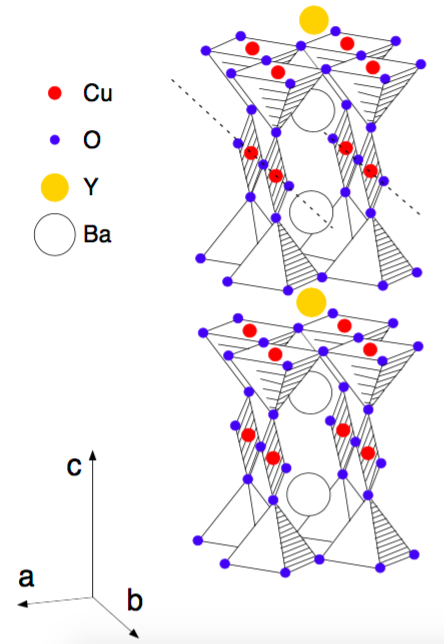
\includegraphics[width=6cm]{supercond.png}
\caption{Crystal structure of YBa$_2$Cu$_3$O$_{7-\mathrm{\delta}}$}
\end{figure}


\chapter{Experimental setup and Procedure}

The setup consists of four main parts \footnote{\url{http://www.physik.uzh.ch/data/peter/FestkoerperPhysik/InfoPraktFestkoerperphysik.shtml}}\\
\begin{itemize}
\item The specimen holder.\\
This is the container where the superconductor is placed. There are connections for the temperature sensor, the heating foil and for the resistance measurement.\\
\item The cryostat.\\
This part serves as a temperature regulator. The sample is enclosed in a tube, which is submerged in liquid nitrogen. To keep the sample at a certain temperature, a heating foil is attached behind the sample. This heating foil is needed, as liquid nitrogen has a constant temperature of around 77K at atmospheric pressure. \\
\item The vacuum system.\\
A vacuum of $2.8 \cdot 10^{-3}$mbar was created inside the tube. This vacuum helps to reduce the heat transfer between the probe and its surroundings, as heat is primarily exchanged through convection.\\ 
\item The electromagnet.\\
The tube with the sample is placed inside an electromagnet. Therefore the experiment can be repeated with different magnetic fields up to a field of 0.8T . 

\end{itemize}

\section*{Procedure}

The first step in the measuring process is the cooling. The sample and the apparatus are cooled by liquid nitrogen which gets pumped into the system. With the heating foil and the PID-controller a arbitrary temperature within the apparatus working range can be achieved. In the experiment the starting temperature was set to 82K. When this temperature was reached and stabilized the heating and cooling got turned off and the experiment started. While the samples temperature slowly increased due to the temperature difference to the room temperature, we measured the resistivity. 
Since the sample is in a vacuum, the rise in temperature happens very slowly and we can assume the sample to be in thermal equilibrium. 

The resistivity measurement got realised in a four point measuring circuit. This setup is usually used when a resistance has to be measured precisely. 

\begin{figure}[H]
\centering
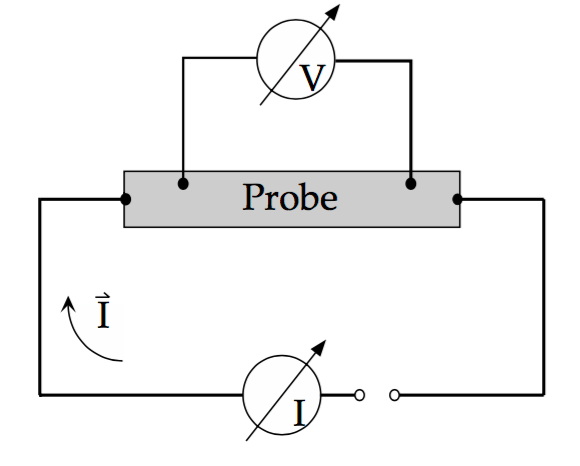
\includegraphics[width=6cm]{vierpunkt.png}
\caption{The four-point measuring technique}
\label{vierpunkt}
\end{figure}


Another measuring technique got used which at first glance may seem rather unusual. The direction of the current got reversed after each measurement. We can think of this as running the current in figure \ref{vierpunkt} first in clockwise direction and than in counterclockwise.

The reason behind this procedure are the contact potentials (also known as \emph{Volta potential}) of the plugs. Every connection between two different metals leads to such a potential and therefore creates a systematic error. To reduce this systematic error we computed the final resistivity as the mean between the clockwise-resistance and the counterclockwise-resistance.  


\chapter{Results}

\begin{framed}
\begin{table}[H]
\centering
\renewcommand{\arraystretch}{1.2} % Abstandzwischen Zeilen
\setlength{\tabcolsep}{3mm} % Abstandzwischen Spalten
\footnotesize
\begin{tabular}{r|ccc}
$B[T]$ & 0 & 0.42 & 0.7 \\ 
\hline 
$T_{c} [K]$ & 94.3 $\pm$ 0.4 & 94.0 $\pm$ 0.4 & 94.1 $\pm$ 0.5 \\ 
\end{tabular}
\caption[]{Results}
\end{table} 
\end{framed}





\begin{figure}[H]
\centering
\includegraphics[scale=0.5]{Widerstand}
\caption[]{Measurement of the mean resistance.}
\end{figure}

\section{Questions}

\begin{enumerate}

\item Does YBa$_2$Cu$_3$O$_{7-\mathrm{\delta}}$  behave like a metal above the transition temperature? Describe the temperature dependence qualitatively.\\
\\
In the measured region just above the transition temperature, the resistance increases linearly with respect to the temperature. This corresponds to the expected behaviour of a metal.  

\item What is the expected dependence of the resistance of a metal (no superconductivity) due to an external magnetic field (for small magnetic fields)?\\
\\
For small magnetic fields, the resistance of a metal is independent due to an external magnetic field. The reason behind this is the Hall-effect. The magnetic field causes a Lorentz-force, acting on all moving electrons, perpendicular to the magnetic filed and the direction of the electrons velocities. Therefore the electrons concentrate on one side of the metal and an electric field, in the direction of the Lorentz-force is set up. This causes a force on the electrons, in the opposite direction. As soon as the equilibrium is reached, where the two forces are equal, the electrons are able to move like if there was no magnetic field. Therefore, the resistance is the same. 

\item Determine the transition temperature, $T_c$. How do you do this?\\
\\
Hauptidee Bericht

\item Why is the resistance measurement carried out twice with a reversion of the polarity?\\
\\
Kontaktspannung, richtungsabhängig

\end{enumerate}

\chapter{Error calculus}

\section{Derivative}

Since the measurement more or less looks like a step-function one can get the error of $T_{c}$ by looking at the width of the derivative-curve. In an ideal case the derivative of a step-function would give a $\delta$-function which is localised in one point. Since the measured data has a lot of noise on top of the underling curve, we had to use the so called \emph{five-point-stencil method \footnote{\url{https://en.wikipedia.org/wiki/Five-point_stencil}}} to compute the derivative. Otherwise we wouldn't see the peak we are looking for. 

The \emph{five-point-stencil method} takes not only the next date point into account but also the 4 surrounding values. With this method we get a more smooth and useful curve. 

$$f'(x) \approx \frac{-f(x+2 h)+8 f(x+h)-8 f(x-h)+f(x-2h)}{12 h}$$

\begin{figure}[H]
\centering
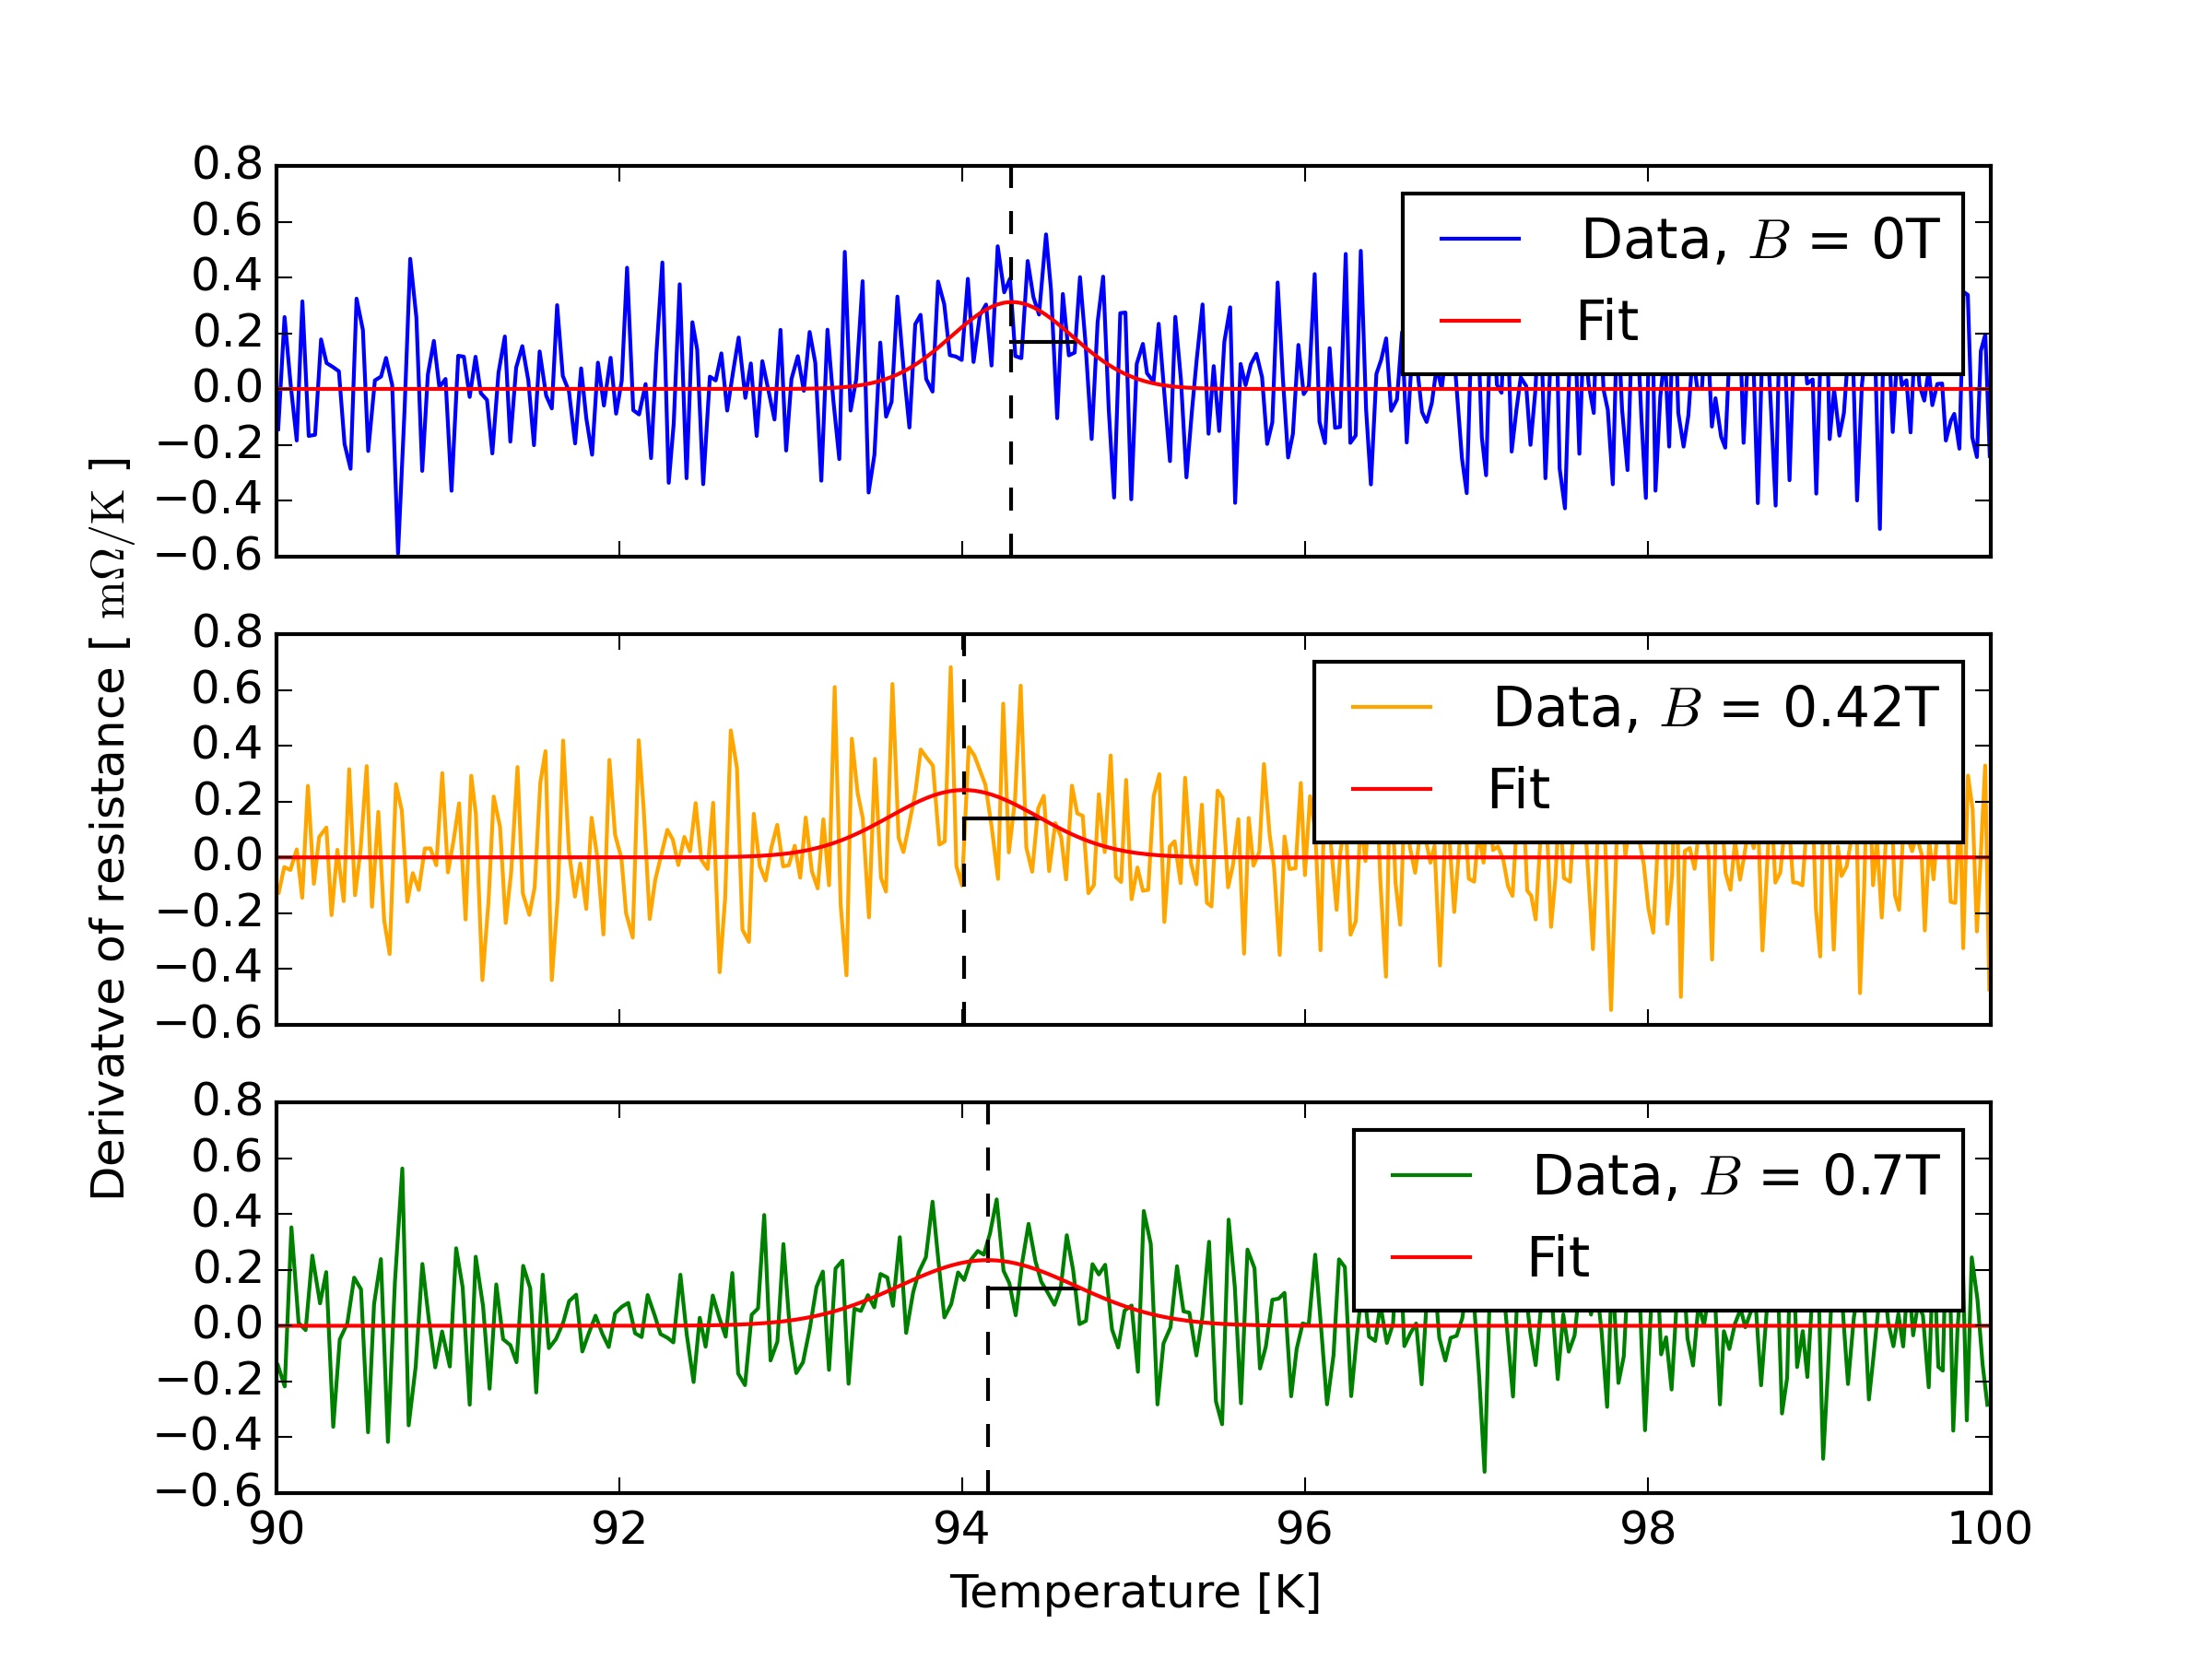
\includegraphics[scale=0.11]{Criticaltemperature3}
\caption[]{Derivative calculated using the five-point stencil method and considering the direct neighbours (h=1).  }
\end{figure}

\begin{figure}[H]
\centering
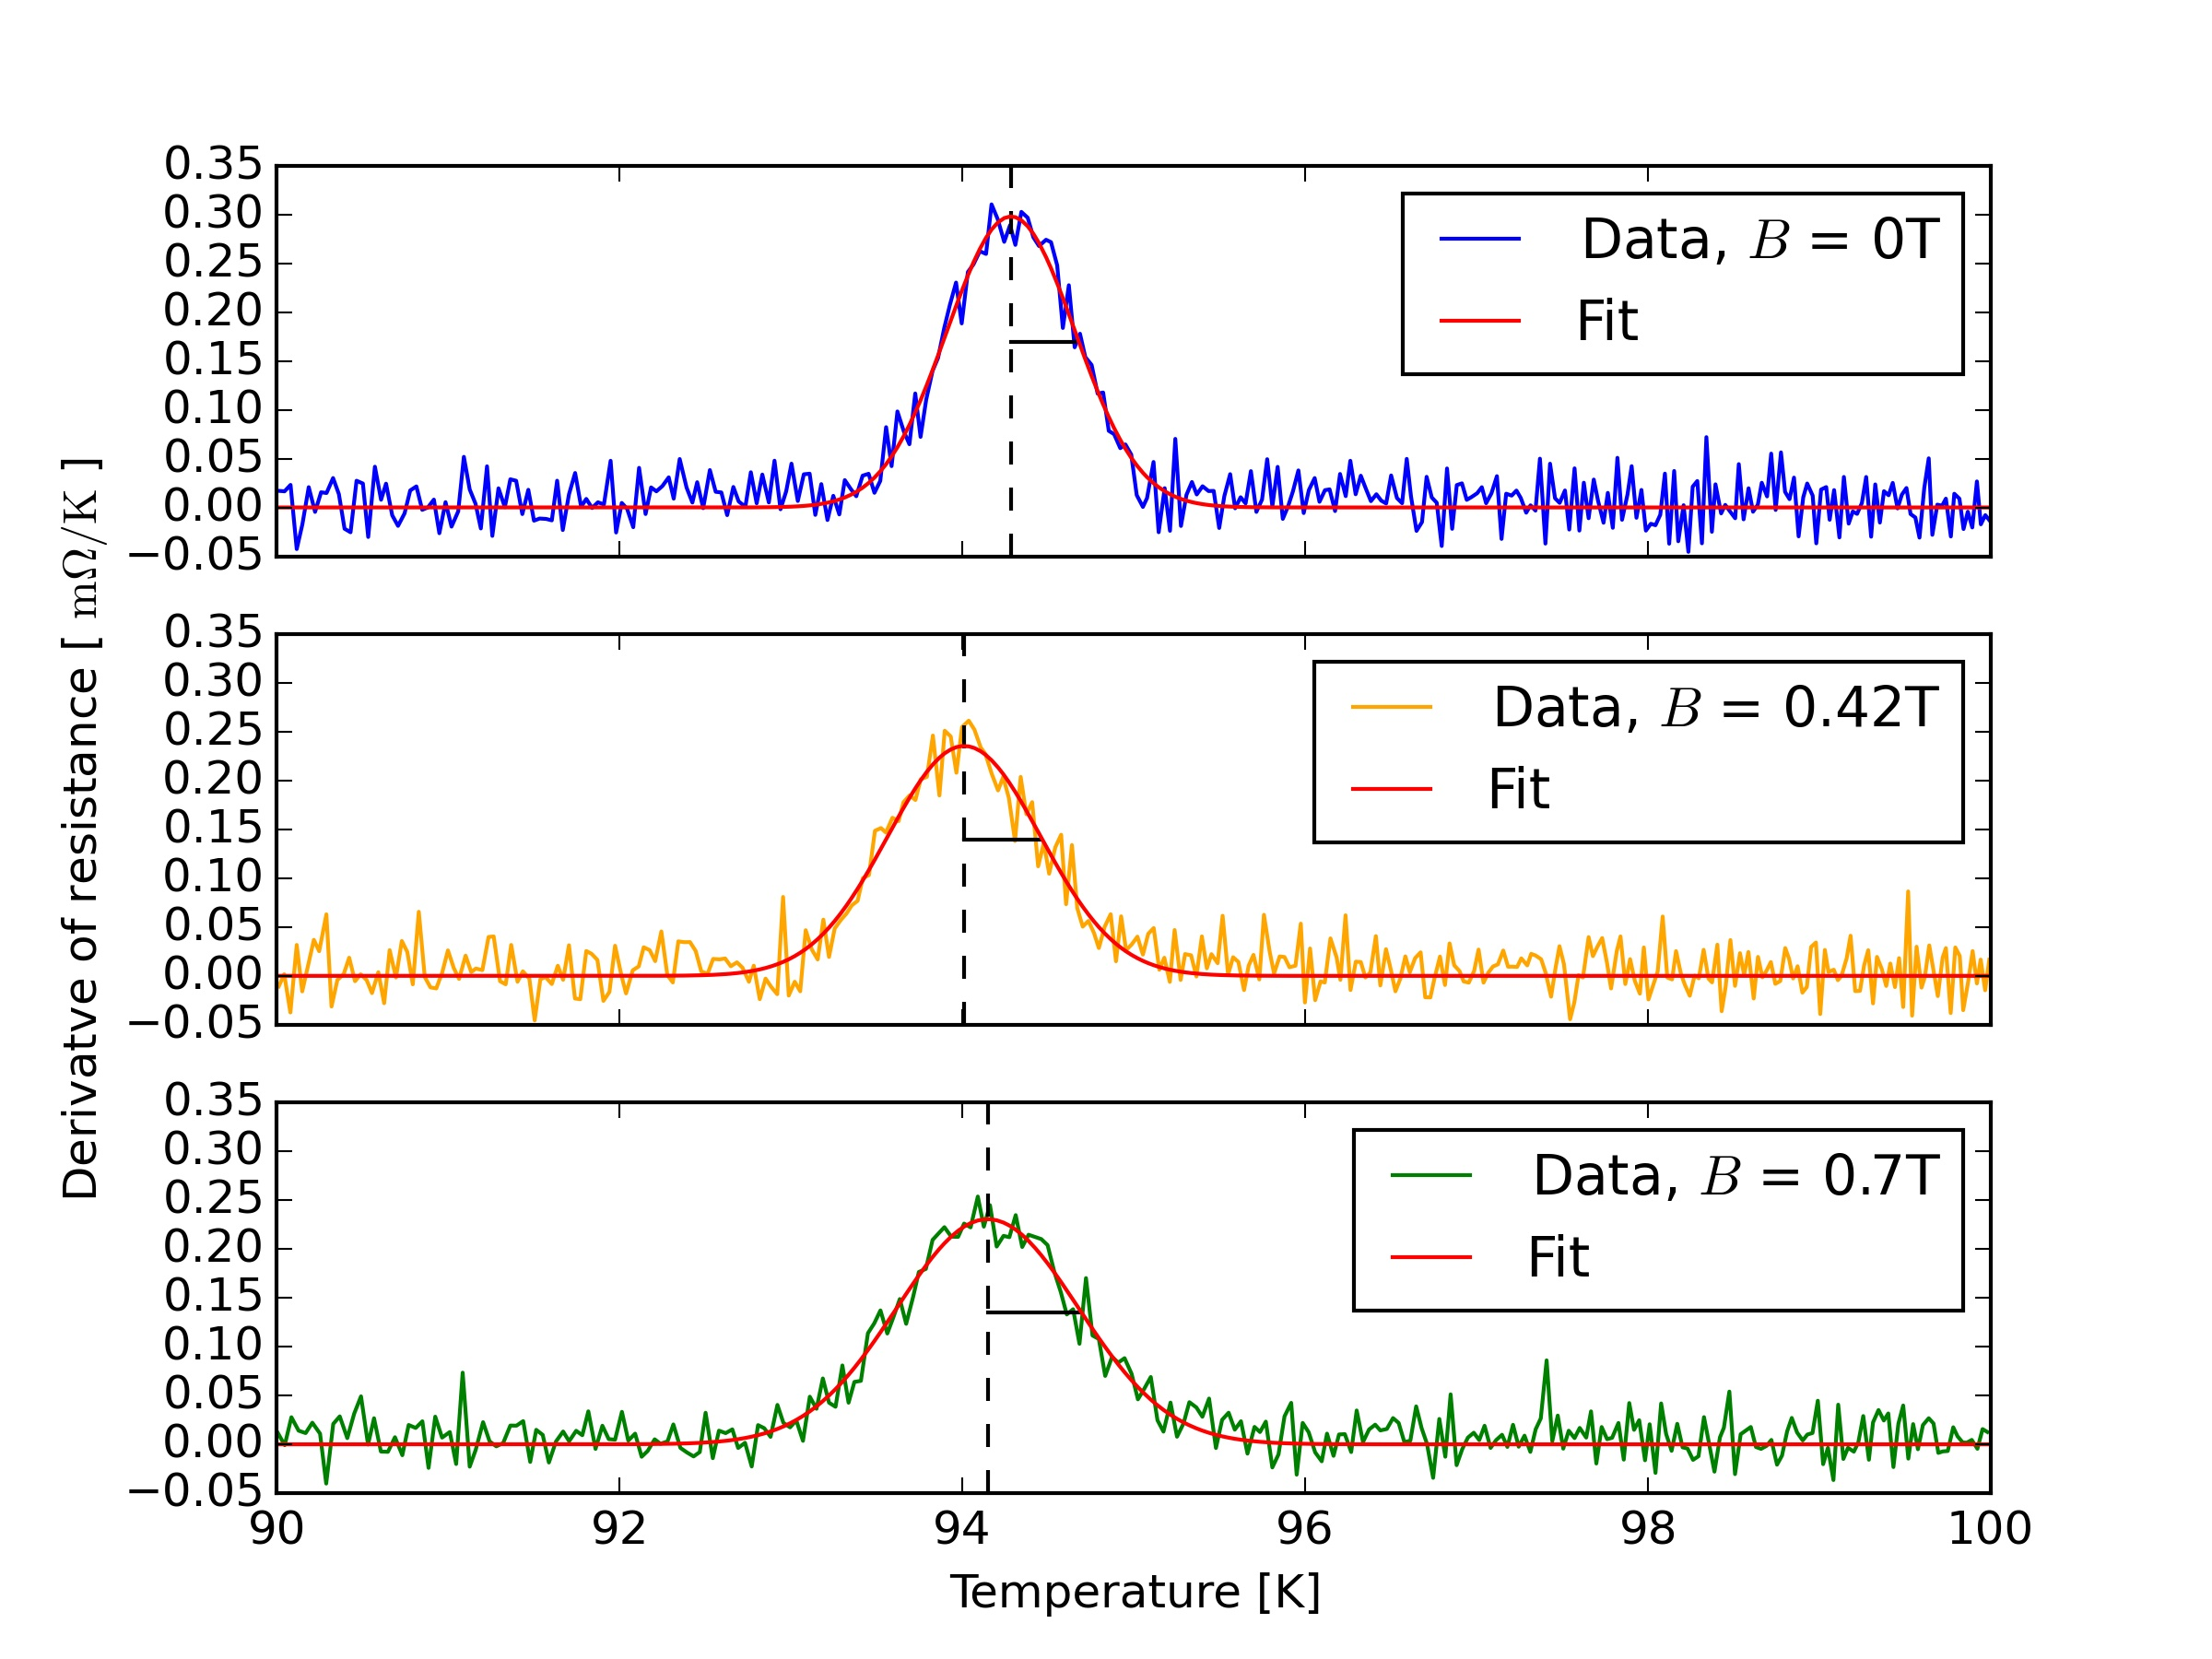
\includegraphics[scale=0.11]{Criticaltemperature2}
\caption[]{Derivative calculated with h=10.}
\end{figure}





\end{document}
